\chapter{Implementation}\label{ch:implementation}

All the code for this implementation can be found in the GitHub repository \cite{github-repo}.
It is structured in preprocessing and \ac{lstm} implementation, which will be described in the following sections.

\section{Preprocessing}
As described in \Cref{ch:data-ana}, the data was prepared and has the following structure:
The first column contains the \ac{wifi} timestamps in milliseconds, the second and third columns contain the waypoint data values x and y in meters, the fourth to sixth columns contain the acceleration data values x, y, and z in meters per second squared, and the rest of the columns contain the \ac{rssi} data for each \ac{bssid} in the dataset.
This data is preprocessed for the model as follows:\\
First, I set a \texttt{window\_size} for the sliding window I want to use for the model, as \ac{lstm} needs sequence data.
According to Ja{\'e}n-Vargas et al. \cite{EffectsSlidingWindow2022}, the sliding window size for acceleration-based activity recognition should be \(25 * 0.25 = 6.25\) seconds, so I choose \(3\) as the sliding window size, as our dataset has \ac{wifi} timestamps for every about 2 seconds.
If a file has less or equal to \(3\) lines, it will not be used because I cannot apply a sliding window for this data.
Furthermore, the length of each file will be saved to know where I need to split the sliding window in the preprocessing later.
Then, I create our target variable, which is a variable where the \ac{bssid} with the highest \ac{rssi} is saved for each timestamp, which results in a list with 4795 entries, as there are 4795 \acp{bssid} in our dataset.
An encoding of the target variable is necessary for the model, so I encode the target variable with a one-hot encoding.
I initialize a \texttt{MinMaxScaler} which ranges from \(-1\) to \(1\), as \acp{lstm} use \texttt{tanh} as activation function. 
Furthermore, our model needs to scale the \ac{rssi} values so that the \ac{rssi} values are considered in the learning process.
By ensuring all \ac{rssi} features have similar scales, the learning process can be more stable and faster. 

After this, I use the \texttt{window\_size} to create sequences with our files.
If the length of the file mentioned above is reached, a stop in creating the sequences for this file is done, and the next sequences will be created out of the next file.
There are 
\[S = \texttt{Length of file} - \texttt{window\_size} + 1\] 
sequences per file, which results in 

\[
    S_{\text{total}} = \sum_{i=0}^{146} (\text{Length of } i^{\text{th}} \text{ file} - \text{window\_size} + 1)
\]
sequences in total.

I shuffle the data to eliminate chronological biases. 
Instead of a basic train-test split, I use 5-fold cross-validation.
This trains the model on 4 partitions and tests on the remaining one, ensuring a comprehensive evaluation.
A k-value of 5 is standard in machine learning due to its balance between computational efficiency and robust evaluation across varied data subsets.

\begin{figure}[h]
    \centering
    \begin{tikzpicture}

% File representation
\draw[blue] (2,1) rectangle (7,9);
\draw[blue] (2,7) -- (7,7);
\node[align=center, blue, font=\small] at (6.25, 7.25) {File 1};
\draw[blue] (2,4) -- (7,4);
\node[align=center, blue, font=\small] at (6.25, 4.25) {File 2};
\draw[blue] (2,2) -- (7,2);
\node[align=center, blue, font=\small] at (6.25, 2.25) {...};
\draw[blue] (2,1) -- (7,1);
\node[align=center, blue, font=\small] at (6.25, 1.25) {File 147};
\node[align=center, font=\small] at (4.5, 9.5) {File with data of the whole floor};

% Arrow
\draw[->, thick] (7.5,5) -- (9.5,5);

% Sliding window representation
\draw[green] (2,8.5) rectangle (7,9);
\node[align=center, green, font=\small] at (4.5, 8.25) {Sliding Window};

% Generated sequences representation
\draw[orange] (10,3.5) rectangle (15,9);
\draw[orange] (10,7.5) -- (15,7.5);
\node[align=center, orange, font=\small] at (14.25, 7.75) {File 1};
\draw[orange] (10,5.5) -- (15,5.5);
\node[align=center, orange, font=\small] at (14.25, 5.75) {File 2};
\draw[orange] (10,4) -- (15,4);
\node[align=center, orange, font=\small] at (14.25, 4.25) {...};
\draw[orange] (10,3.5) -- (15,3.5);
\node[align=center, orange, font=\small] at (14.25, 3.75) {File 147};
\node[align=center, orange, font=\small] at (12.5, 9.5) {Generated Sequences};

\end{tikzpicture}
    
    \caption{Size of sequence generation for all files}
    \label{fig:sequence_generation}
\end{figure}


\section{\ac{lstm} Tuning, Training and Testing}

I test different models with keras-tuner \cite{keras_tuner} \texttt{RandomSearch} with different hyperparameters.
As a \ac{lstm} model needs at least one \ac{lstm} layer, the number of layers must be set, which is one hyperparameter of the model.
The first LSTM layer's architecture is contingent upon the potential presence of a subsequent LSTM layer, and it gets the number of samples, timesteps, and features.
If there will be a second LSTM layer, the first LSTM must return sequences to feed the subsequent layer.
This conditional structure provides flexibility in model depth.
The activation function for the LSTM layers will be \texttt{tanh} as it is a traditional choice.
A Dropout layer can be optionally added, to randomly select neurons to be ignored during training, helping prevent overfitting, which was mentioned in \Cref{ch:discuss-ml}.
A Batch Normalization layer can also be optionally added.
Batch normalization standardizes the activations of a given input volume before passing it to the next layer, helping improve the model's convergence speed and overall accuracy.
The final layer is a Dense layer with a \texttt{softmax} activation function, which is needed for multi-class classification problems to get the probabilities for each class \cite{cat_cross_entropy}.
As optimizers the \texttt{RandomSearch} will try out \texttt{Adam}, \texttt{SDG}, and \texttt{RMSprop} with adapted learning rates, which are used to minimize the loss function.
If a learning rate should not be set, the default learning rate for each of the optimizers is \(0.001\).

Finally, the model is compiled and tested with the chosen optimizer and the loss function \texttt{categorical\_crossentropy}, which converts the probabilities to target values.

This \texttt{RandomSearch} leads to the following hyperparameters:
\begin{itemize}
    \item lstm\_units: 512
    \item second\_lstm\_layer: False
    \item dropout: True with rate 0.3
    \item batch\_norm: True
    \item learning\_rate: False
    \item optimizer: sgd
    \item batch\_size: 96
\end{itemize}

When configured with the parameters mentioned above, the model is shown in \Cref{final_model}.
\begin{figure}[h!]
    \centering
    \begin{tikzpicture}[
    node distance=3cm,
    block/.style={rectangle, draw, fill=blue!20, text width=7em, text centered, rounded corners, minimum height=4em},
    line/.style={draw, -{Latex[length=2mm]}},
]

% Nodes
\node (input) {Input}; %\\ $3 \times 4975$ does not work
\node [block, right of=input] (lstm) {LSTM\\Units: 512\\Optimizer: sgd\\Batch Size: 96};
\node [block, right of=lstm] (dropout) {Dropout Layer\\Rate: 0.3};
\node [block, right of=dropout] (batchnorm) {Batch Normalization};
\node [block, right of=batchnorm] (output) {Output (Dense layer)\\softmax\\};

% Paths
\path [line] (input) -- (lstm);
\path [line] (lstm) -- (dropout);
\path [line] (dropout) -- (batchnorm);
\path [line] (batchnorm) -- (output);

\end{tikzpicture}

    \caption{The final model architecture.}
    \label{final_model}
\end{figure}


% \begin{figure}[h!]
%     \centering
%     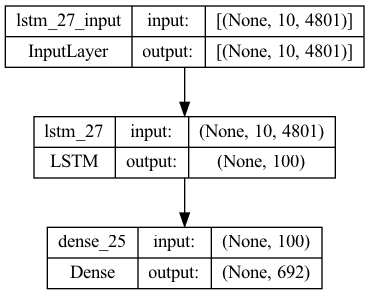
\includegraphics[scale=0.5]{images/model_plot.png}
%     \caption{An example LSTM Network with Input, LSTM, and Dense Layer with 4801 Features and window\_size of 10.}
%     \label{fig:lstm_architecture}
% \end{figure}

%\noindent
